\documentclass[10pt,a4paper,twocolumn]{article}

% --- Page Geometry & Two-Column Grid ---
\usepackage[a4paper, left=1.72cm, right=1.72cm, top=1.95cm, bottom=1.90cm, headheight=15pt, headsep=9pt, footskip=18pt]{geometry}
\setlength{\columnsep}{0.66cm}

% --- Classic Academic Serif Typography (Palatino + True Small Caps) ---
\usepackage[T1]{fontenc}
\usepackage[utf8]{inputenc}
\usepackage{lmodern}
\linespread{1.05}
\renewcommand{\ttdefault}{lmtt}
\usepackage[protrusion=true,expansion=true]{microtype}

% --- Core Academic Packages ---
\usepackage{amsmath}
\usepackage{amssymb}
\usepackage{booktabs}
\usepackage{array}
\usepackage{tabularx}
\usepackage{graphicx}
\usepackage{xcolor}
\usepackage{enumitem}
\usepackage{titlesec}
\usepackage{fancyhdr}
\usepackage{caption}
\usepackage{hyperref}

% --- Strictly Monochrome Palette (Pure Black & Neutral Grays; Zero Color) ---
\definecolor{ink}{HTML}{111111}
\definecolor{muted}{HTML}{555555}
\definecolor{rulelight}{HTML}{BDBDBD}
\definecolor{ruledark}{HTML}{222222}

\hypersetup{
  colorlinks=true,
  linkcolor=ink,
  urlcolor=ink,
  citecolor=ink,
  pdftitle={Predicting Formula 1 Points Finishes (2010-2024): A Temporal Ablation},
  pdfauthor={Marc Font Hostalet, David Redrejo Perez, Elias Barreiro Pena}
}

% --- Classic Academic Section Hierarchy (No Colored Underlines) ---
\titleformat{\section}
  {\normalsize\bfseries\color{ink}}
  {\thesection.}{0.5em}{}
\titleformat{\subsection}
  {\fontsize{9.4pt}{11.2pt}\selectfont\bfseries\itshape\color{ink}}
  {\thesubsection}{0.45em}{}
\titlespacing*{\section}{0pt}{10pt plus 2.5pt minus 1.5pt}{3.8pt plus 1pt}
\titlespacing*{\subsection}{0pt}{7pt plus 1.5pt minus 1pt}{2.5pt plus 0.5pt}

% --- Paragraphs, Lists, Widow/Club Control & Inline Code ---
\setlength{\parindent}{1em}
\setlength{\parskip}{1.2pt plus 0.4pt}
\setlength{\emergencystretch}{1.6em}
\widowpenalty=10000
\clubpenalty=10000
\setlist[itemize]{itemsep=1.8pt, parsep=0pt, topsep=3pt, leftmargin=1.2em, label=\textbullet}
\setlist[enumerate]{itemsep=1.8pt, parsep=0pt, topsep=3pt, leftmargin=1.35em}
\newcommand{\code}[1]{{\fontsize{8.5pt}{10pt}\selectfont\ttfamily #1}}
\newcommand{\ub}{\_\allowbreak{}}
\newcolumntype{L}{>{\raggedright\arraybackslash}X}

% --- Captions (Unified Classic Serif; Tables Top, Figures Bottom) ---
\captionsetup{
  font=footnotesize,
  labelfont=bf,
  textfont=normalfont,
  labelsep=period,
  skip=4pt
}
\captionsetup[table]{position=top, skip=4pt}
\captionsetup[figure]{position=bottom, skip=4pt}

% --- Two-Column Float Tuning ---
\renewcommand{\topfraction}{0.88}
\renewcommand{\dbltopfraction}{0.88}
\renewcommand{\bottomfraction}{0.80}
\renewcommand{\textfraction}{0.08}
\renewcommand{\floatpagefraction}{0.78}
\renewcommand{\dblfloatpagefraction}{0.78}
\setcounter{topnumber}{3}
\setcounter{dbltopnumber}{3}
\setcounter{totalnumber}{5}
\setlength{\dbltextfloatsep}{10pt plus 2.5pt minus 2pt}
\setlength{\dblfloatsep}{8pt plus 2pt minus 2pt}
\setlength{\textfloatsep}{8pt plus 2pt minus 2pt}
\setlength{\intextsep}{7pt plus 2pt minus 2pt}

% --- Running Headers & Footers (Monochrome Classic Style) ---
\pagestyle{fancy}
\fancyhf{}
\lhead{\scriptsize\scshape\color{muted} Predicting Formula 1 Points Finishes (2010--2024)}
\rhead{\scriptsize\scshape\color{muted} Fundamentals of Machine Learning (UAB) \;\textbar\; Team 05}
\cfoot{\footnotesize\color{muted}\thepage\ / 5}
\renewcommand{\headrulewidth}{0.4pt}
\renewcommand{\headrule}{\hbox to\headwidth{\color{rulelight}\leaders\hrule height \headrulewidth\hfill}}
\renewcommand{\footrulewidth}{0pt}

\fancypagestyle{bodyfirst}{
  \fancyhf{}
  \cfoot{\footnotesize\color{muted}\thepage\ / 5}
  \renewcommand{\headrulewidth}{0pt}
}

\begin{document}

% =========================================================================
% DEDICATED MONOCHROME ACADEMIC FRONT PAGE (UNNUMBERED)
% =========================================================================
\begin{titlepage}
  \thispagestyle{empty}
  \color{ink}
  \centering

  % Top Institutional Masthead
  \vspace*{0.4cm}
  {\normalsize\scshape\textls[110]{Autonomous University of Barcelona (UAB)}}\\[4pt]
  {\small\color{muted} Fundamentals of Machine Learning \;\textperiodcentered\; Academic Year 2026--2027}\\[3pt]
  {\footnotesize\scshape\textls[90]{\color{muted} Final Project Report \;\textemdash\; Project Team 05}}

  \vspace{0.55cm}
  {\color{ruledark}\hrule height 0.9pt}
  \vspace{2pt}
  {\color{rulelight}\hrule height 0.4pt}

  % Title & Subtitle
  \vspace{1.8cm}
  {\fontsize{20pt}{24.5pt}\selectfont\bfseries Predicting Formula 1 Points Finishes\\[4pt] (2010--2024)\par}
  \vspace{0.55cm}
  {\fontsize{12pt}{15.5pt}\selectfont\itshape\color{muted}
    A Temporal Ablation of Qualifying Position, Rolling Constructor Momentum,\\
    and Historical Circuit Affinity\par}

  \vspace{1.35cm}
  {\color{rulelight}\rule{0.32\textwidth}{0.5pt}}
  \vspace{1.1cm}

  % Authors & Supervision Block
  {\footnotesize\scshape\textls[100]{\color{muted} Authors}}\\[8pt]
  {\large
    Marc Font Hostalet \quad\textperiodcentered\quad
    David Redrejo P\'erez \quad\textperiodcentered\quad
    Elias Barreiro Pena
  }\\[16pt]

  {\footnotesize\scshape\textls[100]{\color{muted} Instructors}}\\[5pt]
  {\normalsize Oguz Mulayim \quad\textperiodcentered\quad D. Karatzas}

  \vspace{1.5cm}

  % Classic Centered Academic Abstract (No Colored Boxes)
  \begin{minipage}{0.88\textwidth}
    {\color{ruledark}\hrule height 0.6pt}
    \vspace{10pt}
    \begin{center}
      {\small\scshape\bfseries\textls[120]{Abstract}}
    \end{center}
    \vspace{2pt}
    {\fontsize{9.2pt}{12.4pt}\selectfont
    \noindent Formula 1 race outcomes combine deterministic car-and-driver pace with high-variance stochastic incidents. Using the relational Ergast/Kaggle Formula 1 database restricted to the unified Top-10 points era (\textbf{2010--2024}, 305 Grands Prix, $n=6{,}436$, 47.4\% Top-10 rate), we engineer \textbf{26 strictly pre-race features} partitioned into three disjoint factor groups---\textbf{Qualifying \& Grid (A)}, \textbf{Rolling Constructor \& Driver Momentum (B)}, and \textbf{Historical Circuit Characteristics (C)}---under automated zero-leakage guarantees and strict season-based temporal evaluation (\textbf{Development:} 2010--2021 with 5-fold expanding-window CV on 2017--2021; \textbf{Held-Out Test:} 2022--2024 Ground-Effect era, $n=1{,}359$). Across 9 curriculum algorithms, regularized linear models significantly beat the scrubbed \code{grid <= 10} heuristic (\textbf{77.12\%} test accuracy): \textbf{L2 Logistic Regression} reaches \textbf{80.43\%} ($+3.31$ pp, McNemar $p=0.0012$, ROC-AUC \textbf{0.8708}), \textbf{L1 Logistic} wins temporal CV (\textbf{0.8401} AUC) and statistically ties \textbf{Random Forest} on Test (McNemar $p=1.000$), and \textbf{Linear SVM} achieves the best calibration (Log-Loss \textbf{0.4504}). Our centerpiece \textbf{7-subset ablation study} across 5 model families proves that \code{A+B} delivers virtually 100\% of achievable pre-race AUC ($\sim$0.871), whereas adding Circuit History (\code{C}) contributes $\Delta\text{AUC} \in [-0.0002, +0.0025]$ and is completely eliminated (0/7 retained) by CV-optimal L1 Lasso. Post-hoc error decomposition reveals that \textbf{60.7\%} of False Positives arise from unpredictable in-race retirements/DNS, quantifying an irreducible Bayes-error floor.\par}
    \vspace{10pt}
    {\color{ruledark}\hrule height 0.6pt}
  \end{minipage}

  \vfill

  % Reproducible Artifacts & Bottom Institutional Footline
  \begin{minipage}{0.88\textwidth}
    \centering
    {\footnotesize\scshape\textls[80]{\color{muted} Executed Notebooks}}\\[4pt]
    {\footnotesize\color{muted}
      \texttt{notebooks/01\_followup1\_obtain\_scrub\_explore.ipynb} (Delivery 1)\\[1.5pt]
      \texttt{notebooks/02\_followup2\_model\_interpret.ipynb} (Delivery 2)
    }
  \end{minipage}

  \vspace{0.8cm}
  {\color{rulelight}\hrule height 0.4pt}
  \vspace{6pt}
  {\footnotesize\scshape\color{muted} Project Team 05 \hfill Autonomous University of Barcelona (UAB) \hfill 2026--2027}
  \vspace*{0.2cm}
\end{titlepage}

% =========================================================================
% TWO-COLUMN SCIENTIFIC BODY (PAGES 1--5)
% =========================================================================
\setcounter{page}{1}
\thispagestyle{bodyfirst}

% --- Compact Running Title Masthead at Top of Page 1 ---
\twocolumn[{
  \begin{@twocolumnfalse}
    \vspace{-10pt}
    \begin{center}
      {\fontsize{11.5pt}{14pt}\selectfont\bfseries Predicting Formula 1 Points Finishes (2010--2024): A Temporal Ablation of Qualifying Position, Rolling Constructor Momentum, and Historical Circuit Affinity}\\[3.5pt]
      {\footnotesize\color{muted} Project Team 05: Marc Font Hostalet, David Redrejo P\'erez, Elias Barreiro Pena \;\textperiodcentered\; Autonomous University of Barcelona (UAB)}
    \end{center}
    \vspace{2pt}
    {\color{ruledark}\hrule height 0.6pt}
    \vspace{8pt}
  \end{@twocolumnfalse}
}]

% =========================================================================
% SECTION 1
% =========================================================================
\section{Introduction \& Objectives}

Predicting whether a Formula 1 driver finishes in the championship points (Top 10) before lights out is a challenging relational tabular classification task governed by longitudinal team development, grid penalties, circuit overtaking geometry, and regulation resets. Public notebooks on the Ergast dataset routinely commit three severe errors: (i)~mixing pre-2010 scoring regimes (Top 5/6/8) with modern Top-10 scoring, (ii)~leaking in-race telemetry (\code{lap\ub times}, \code{pit\ub stops}, target-race \code{status}, or post-race championship standings), and (iii)~applying random train/test splits that leak future car pace backward in time.

To go decisively beyond standard baselines, we enforce an auditable zero-leakage temporal protocol and test three falsifiable hypotheses:
\begin{enumerate}
  \item \textbf{H1 (Factor Group Hierarchy):} Qualifying context (\textbf{Group A}) and rolling constructor/driver momentum (\textbf{Group B}) carry substantially greater predictive weight than historical circuit characteristics (\textbf{Group C}), such that adding \code{C} onto \code{A+B} yields negligible marginal generalization gain.
  \item \textbf{H2 (Regularized Linear Competitiveness):} Regularized linear classifiers (L2/L1 Logistic Regression and Linear SVM) match or rival non-linear kernel and tree ensembles (RBF SVM, Random Forest, Gradient Boosting) on temporally held-out seasons while preserving transparency and superior probability calibration.
  \item \textbf{H3 (Beating the Strong Domain Baseline):} Multi-group pre-race ML models significantly beat the scrubbed \code{grid <= 10} heuristic ($\sim$77\% accuracy), with the largest gains emerging in grid-penalty recoveries and the high-uncertainty midfield transition zone (P8--P13).
\end{enumerate}

% =========================================================================
% SECTION 2
% =========================================================================
\section{Data Description, Scrubbing \& Exploratory Analysis}

\subsection{Relational Schema, Period Restriction (2010--2024) \& Domain Scrubbing}
The Kaggle/Ergast database spans 14 relational CSV tables (1950--2024, 26,759 results). Because FIA scoring rules changed repeatedly (Top~5 in 1950--59, Top~6 in 1960--2002, Top~8 in 2003--09; Figure~\ref{fig:eras}A), restricting modeling targets to \textbf{2010--2024} ensures a uniform Top-10 target (\code{positionOrder <= 10} matches \code{points > 0} with \textbf{0 discrepancies} across \textbf{6,436} entries and 305 Grands Prix) and a balanced \textbf{47.39\%} positive rate. Pre-2010 records (1995--2009) are loaded \emph{strictly} to warm-start prior career starts and historical circuit counts for early 2010 rounds. Scrubbing (\code{src/data.py}) resolves four critical anomalies:

% --- Floats declared on Page 1 -> Top of Page 2 ---
\begin{figure*}[t]
  \centering
  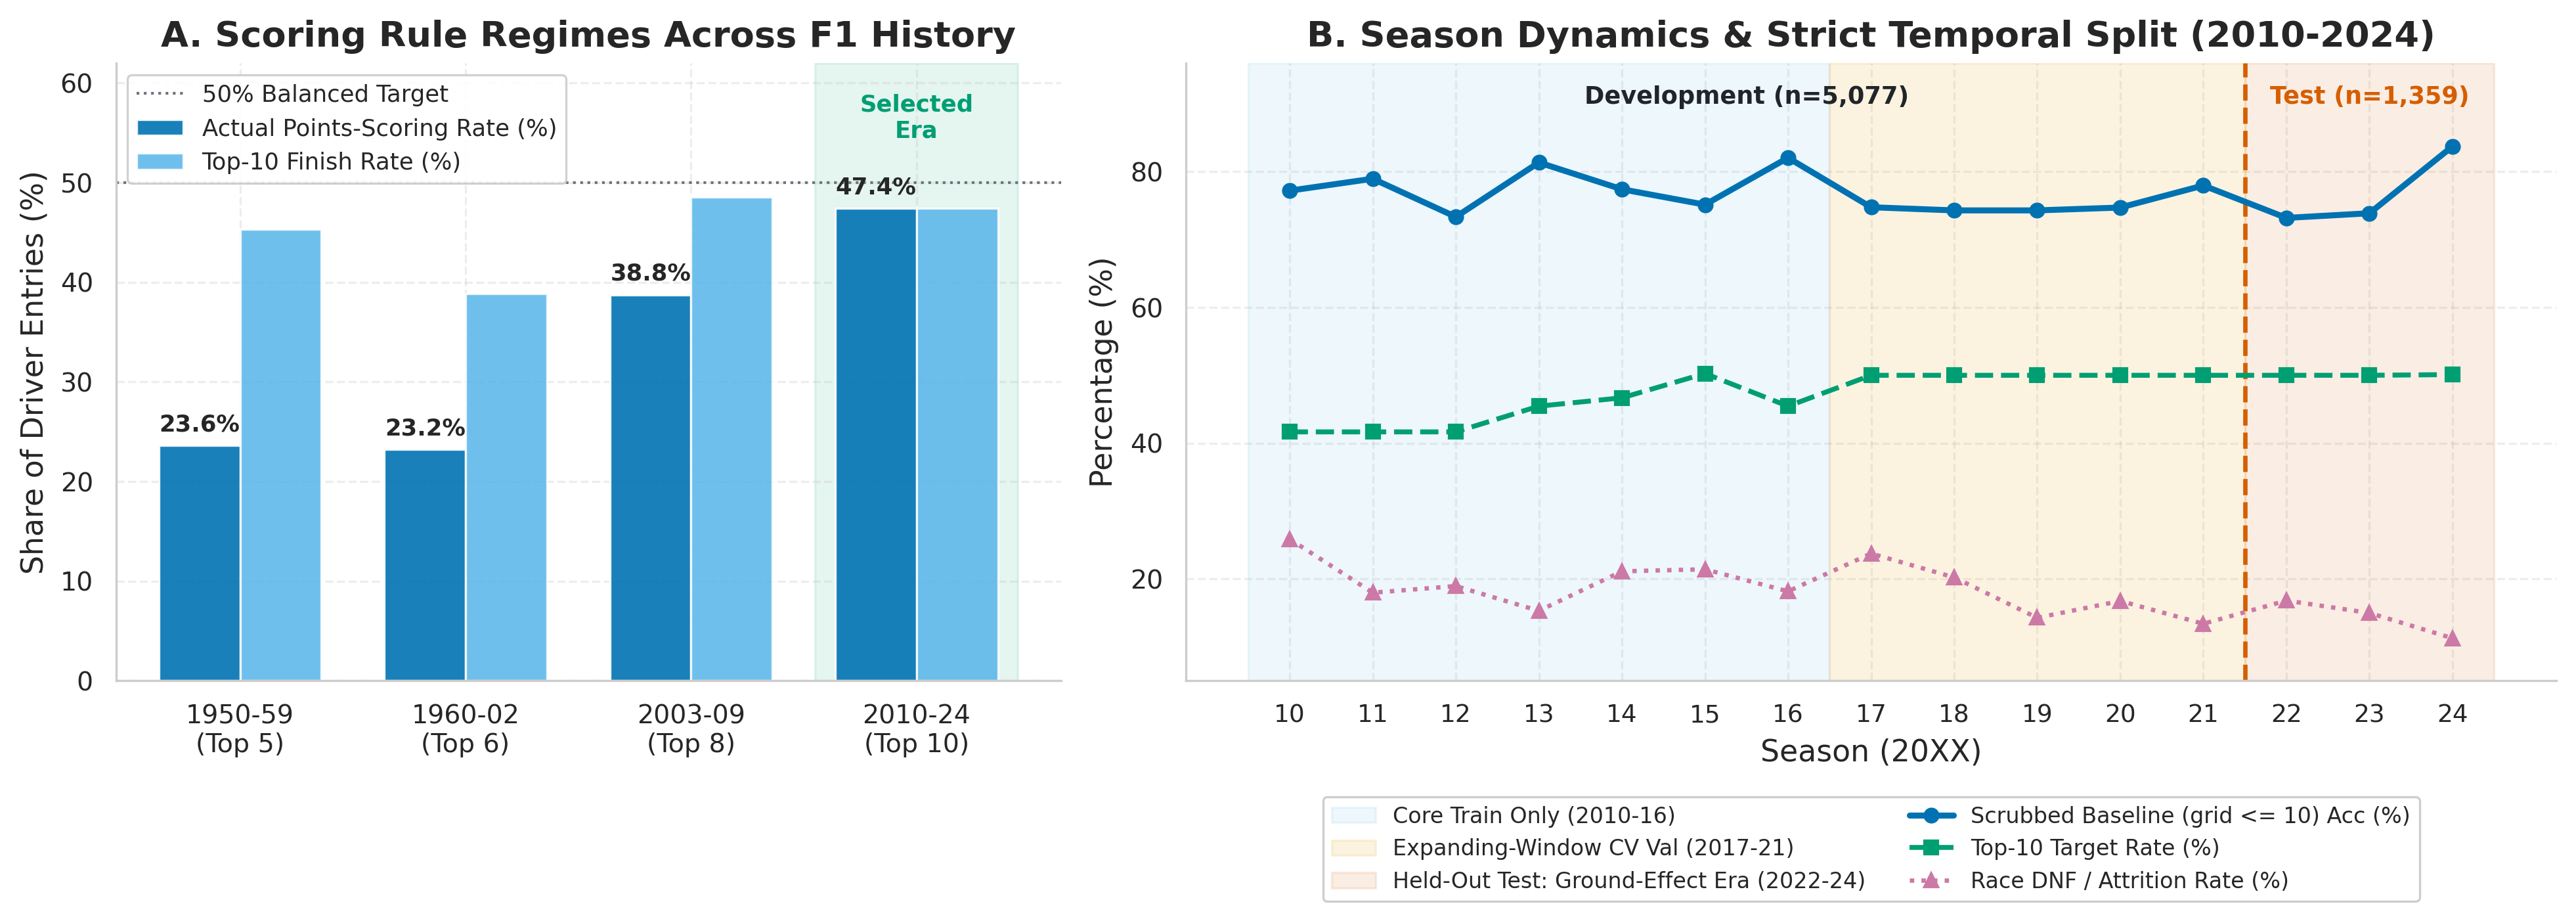
\includegraphics[width=0.92\textwidth]{figures/followup1/fig01_scoring_eras_and_temporal_split.png}
  \caption{FIA scoring regimes justifying restriction to 2010--2024 (A), and strict season-based Development (2010--2021, $n=5{,}077$; 5-fold expanding CV on 2017--2021) vs.\ Held-Out Ground-Effect Test (2022--2024, $n=1{,}359$) protocol (B).}
  \label{fig:eras}
\end{figure*}

\begin{figure*}[t]
  \centering
  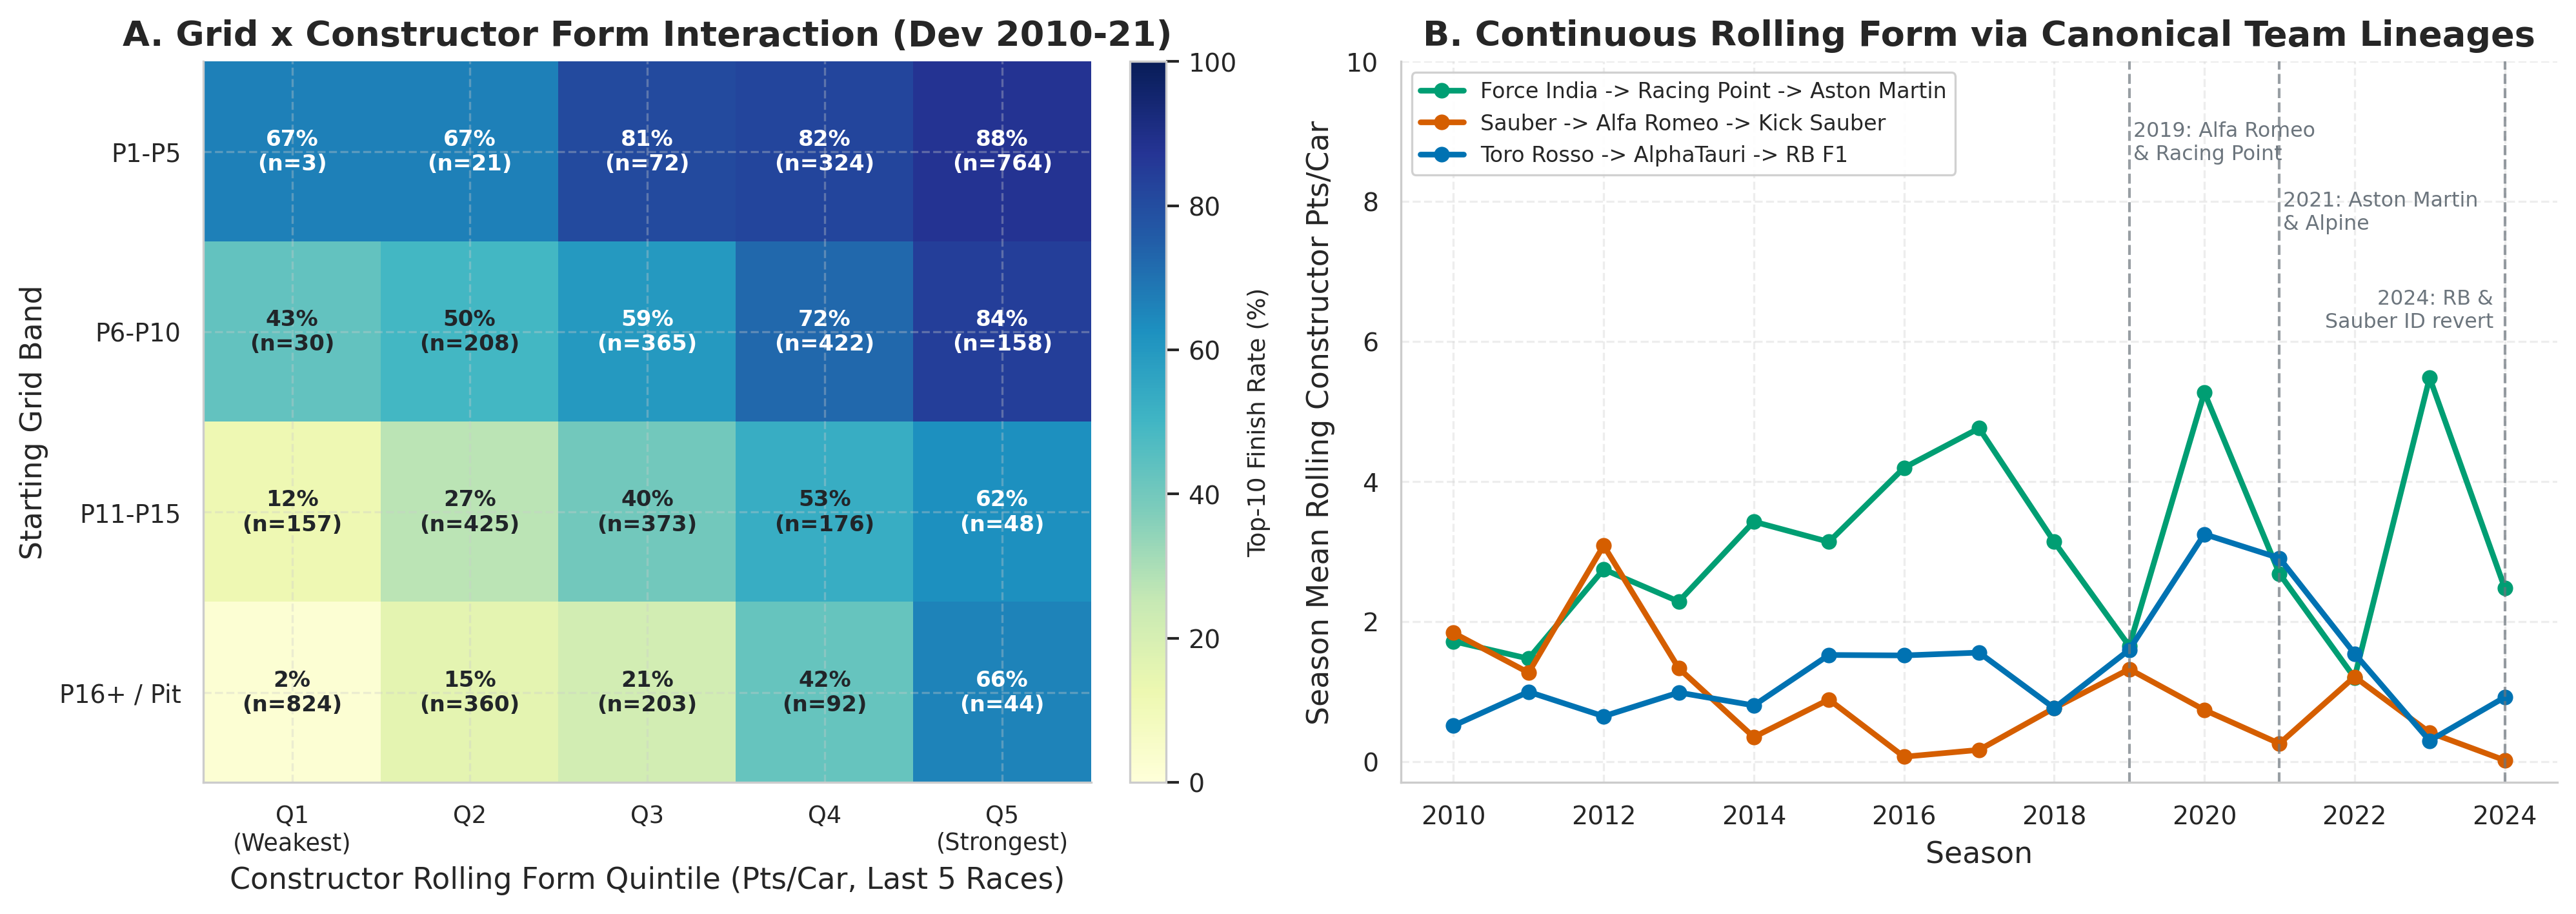
\includegraphics[width=0.91\textwidth]{figures/followup1/fig04_constructor_momentum_and_lineage.png}
  \caption{Grid band $\times$ Constructor rolling form quintile interaction exposing joint separability beyond vertical \code{grid <= 10} (A), and continuous rolling constructor pace restored across team rebrands via canonical lineages (B).}
  \label{fig:form}
\end{figure*}

\begin{table*}[t]
  \centering
  \caption{Univariate discriminative signal (Dev 2010--2021, $n=5{,}077$), mutual information, and multicollinearity across the three disjoint pre-race factor groups.}
  \label{tab:eda}
  {\scriptsize
  \setlength{\tabcolsep}{4.2pt}
  \renewcommand{\arraystretch}{1.15}
  \begin{tabularx}{\textwidth}{l c c l c c L}
    \toprule
    \textbf{Pre-Race Factor Group} & \textbf{\# Feat.} & \textbf{Mean AUC} & \textbf{Max AUC (Top Feature)} & \textbf{Mean MI (nats)} & \textbf{Max VIF} & \textbf{Engineered Feature Summary} \\
    \midrule
    A: Qualifying \& Grid & 8 & 0.7088 & \textbf{0.8419} (\texttt{qualy\_pos}) & 0.1180 & 139.9 & \texttt{grid\_clean}, \texttt{grid\_pct}, \texttt{qualy\_gap\%}, \texttt{teammate\_delta}, \texttt{penalty\_drop} \\
    B: Rolling Form & 11 & \textbf{0.7277} & 0.8346 (\texttt{const\_season\_pts}) & \textbf{0.1282} & 22.2 & 3/5/10-race team \& driver pace, mech DNF, pos gained, career starts \\
    C: Circuit History & 7 & 0.5765 & 0.7044 (\texttt{const\_circ\_top10}) & 0.0288 & 8.4 & Log altitude, prior grid-corr, attrition, EB driver/team circuit affinity \\
    \bottomrule
  \end{tabularx}}
\end{table*}

\begin{itemize}
  \item \textbf{Pit-Lane Starts (\code{grid == 0}, 85 entries):} Raw Ergast codes pit-lane starts/DNS as \code{0}, causing naive \code{grid <= 10} to classify them as pole position (76.03\% acc). Remapping \code{grid == 0} to \code{n\ub entries + 1} plus a pre-race binary flag \code{is\ub pit\ub lane\ub start} raises baseline accuracy by \textbf{+0.89 pp} to \textbf{76.91\%} (Dev: 76.86\%; Test: 77.12\%).
  \item \textbf{Canonical Constructor Lineages (23 raw IDs $\rightarrow$ 13 lineages):} Team rebrands break longitudinal rolling form---notably, Kick Sauber (2024) reverted to ID~15 (2018 Sauber) after five years as Alfa Romeo (ID~51)! Canonicalizing lineages (Force India $\rightarrow$ Racing Point $\rightarrow$ Aston Martin; Toro Rosso $\rightarrow$ AlphaTauri $\rightarrow$ RB; Sauber $\leftrightarrow$ Alfa Romeo; Renault/Lotus $\rightarrow$ Alpine) restores continuous momentum (Figure~\ref{fig:form}B).
  \item \textbf{Missing Qualifying Data (24 rows; 86 Q1 times) \& Strict In-Race Exclusion:} Missing qualifying ranks fall back to scrubbed \code{grid\ub clean}; missing lap gaps are median-imputed strictly inside CV folds. \code{lap\ub times}, \code{pit\ub stops}, target-race \code{status}, race \code{time}/\code{laps}/\code{fastestLap}, and post-race standings are strictly excluded.
\end{itemize}

\subsection{Exploratory Data Analysis (Strictly on Development 2010--2021)}
All exploratory feature-target analyses were strictly confined to Development seasons 2010--2021 ($n=5{,}077$):
\begin{itemize}
  \item \textbf{Midfield Vulnerability \& Joint Separability:} Outside P8--P13, \code{grid <= 10} achieves \textbf{83.55\%}, but plunges to \textbf{59.59\%} inside the \textbf{P8--P13 transition zone} (27.9\% of entries). Top-tier constructors starting P11+ recover to Top-10 \textbf{55--59\%} of the time; Figure~\ref{fig:form}A shows Q5 top teams starting P16+/Pit finish Top-10 \textbf{66\%} of the time vs.\ \textbf{2\%} for Q1 backmarkers, while Q1 teams starting P6--P10 drop to \textbf{43\%}.
  \item \textbf{Univariate Signal \& Multicollinearity (Table~\ref{tab:eda}):} Group~A (max AUC \textbf{0.8419}, \code{qualy\ub pos}) and Group~B (mean AUC \textbf{0.7277}, max \textbf{0.8346}) strongly outperform Group~C (mean AUC \textbf{0.5765}), foreshadowing H1. High within-group VIFs (\code{grid\ub clean}: 139.9; \code{qualy\ub pos}: 104.1; constructor rolling metrics: 13.8--22.2) directly motivate L2/L1 regularization (Lecture~4).
\end{itemize}

% =========================================================================
% SECTION 3
% =========================================================================
\section{Methodology}

\subsection{Leakage-Free Feature Engineering \& Automated Adversarial Audit}
We engineer \textbf{26 pre-race features} partitioned into disjoint Groups \textbf{A (8)}, \textbf{B (11)}, and \textbf{C (7)} (\code{src/features.py}):

% --- Floats declared on Page 2 -> Top of Page 3 ---
\begin{table*}[t]
  \centering
  \caption{Temporal CV (2017--2021) and Held-Out Test (2022--2024, $n=1{,}359$) benchmark across 12 models. McNemar $p$-values test accuracy lift over scrubbed \code{grid <= 10}.}
  \label{tab:bench}
  {\scriptsize
  \setlength{\tabcolsep}{4.6pt}
  \renewcommand{\arraystretch}{1.14}
  \begin{tabularx}{\textwidth}{L l c c c c c c c c}
    \toprule
    \textbf{Model} & \textbf{Family} & \textbf{CV AUC} & \textbf{CV Acc} & \textbf{Test AUC} & \textbf{Test Acc} & \textbf{Test F1} & \textbf{Log-Loss} & \textbf{Brier} & \textbf{McNemar $p$} \\
    \midrule
    Majority Class (Dummy) & Baseline & 0.5000 & 50.00\% & 0.5000 & 49.96\% & 0.0000 & 6.9128 & 0.5004 & --- \\
    \textbf{\texttt{grid <= 10} (Scrubbed)} & Baseline & 0.7520 & 75.20\% & 0.7712 & \textbf{77.12\%} & 0.7708 & --- & --- & \textit{(ref)} \\
    Grid-Only Logistic & Baseline & 0.8186 & 75.20\% & 0.8316 & 77.12\% & 0.7708 & 0.5077 & 0.1651 & --- \\
    \midrule
    \textbf{Logistic Regression (L2, $C=0.1$)} & Linear & 0.8387 & 76.67\% & 0.8708 & \textbf{80.43\%} & 0.7997 & 0.4522 & 0.1437 & \textbf{0.0012} \\
    \textbf{Logistic Regression (L1, $C=0.01$)} & Linear & \textbf{0.8401} & \textbf{76.90\%} & 0.8728 & 79.84\% & 0.7964 & 0.4579 & 0.1450 & \textbf{0.0087} \\
    \textbf{Linear SVM ($C=0.001$, Platt)} & Linear & 0.8376 & 76.23\% & 0.8717 & 79.76\% & 0.7943 & \textbf{0.4504} & \textbf{0.1428} & \textbf{0.0061} \\
    Gaussian Naive Bayes & Prob. & 0.8323 & 76.39\% & 0.8609 & 80.28\% & 0.8027 & 1.5255 & 0.1810 & 0.0017 \\
    k-Nearest Neighbors ($k=75$) & Instance & 0.8290 & 75.17\% & 0.8671 & 80.06\% & 0.8018 & 0.4613 & 0.1467 & 0.0012 \\
    RBF Kernel SVM ($C=0.1, \gamma=0.01$) & Kernel & 0.8365 & 75.94\% & 0.8686 & 80.13\% & 0.8038 & 0.4524 & 0.1432 & $<$0.0001 \\
    Decision Tree (Entropy, $d=4$) & Tree & 0.8201 & 74.65\% & 0.8554 & 78.59\% & 0.7846 & 0.4764 & 0.1513 & 0.2475 \\
    \textbf{Random Forest ($d=5$, leaf 35)} & Ensemble & \textbf{0.8401} & 76.19\% & \textbf{0.8734} & 79.91\% & 0.8020 & 0.4531 & 0.1438 & \textbf{0.0062} \\
    \textbf{Gradient Boosting ($d=2, \text{lr}=0.03$)} & Ensemble & 0.8393 & 76.10\% & 0.8720 & \textbf{81.16\%} & \textbf{0.8153} & 0.4534 & 0.1440 & \textbf{$<$0.0001} \\
    \bottomrule
  \end{tabularx}}
\end{table*}

\begin{figure*}[t]
  \centering
  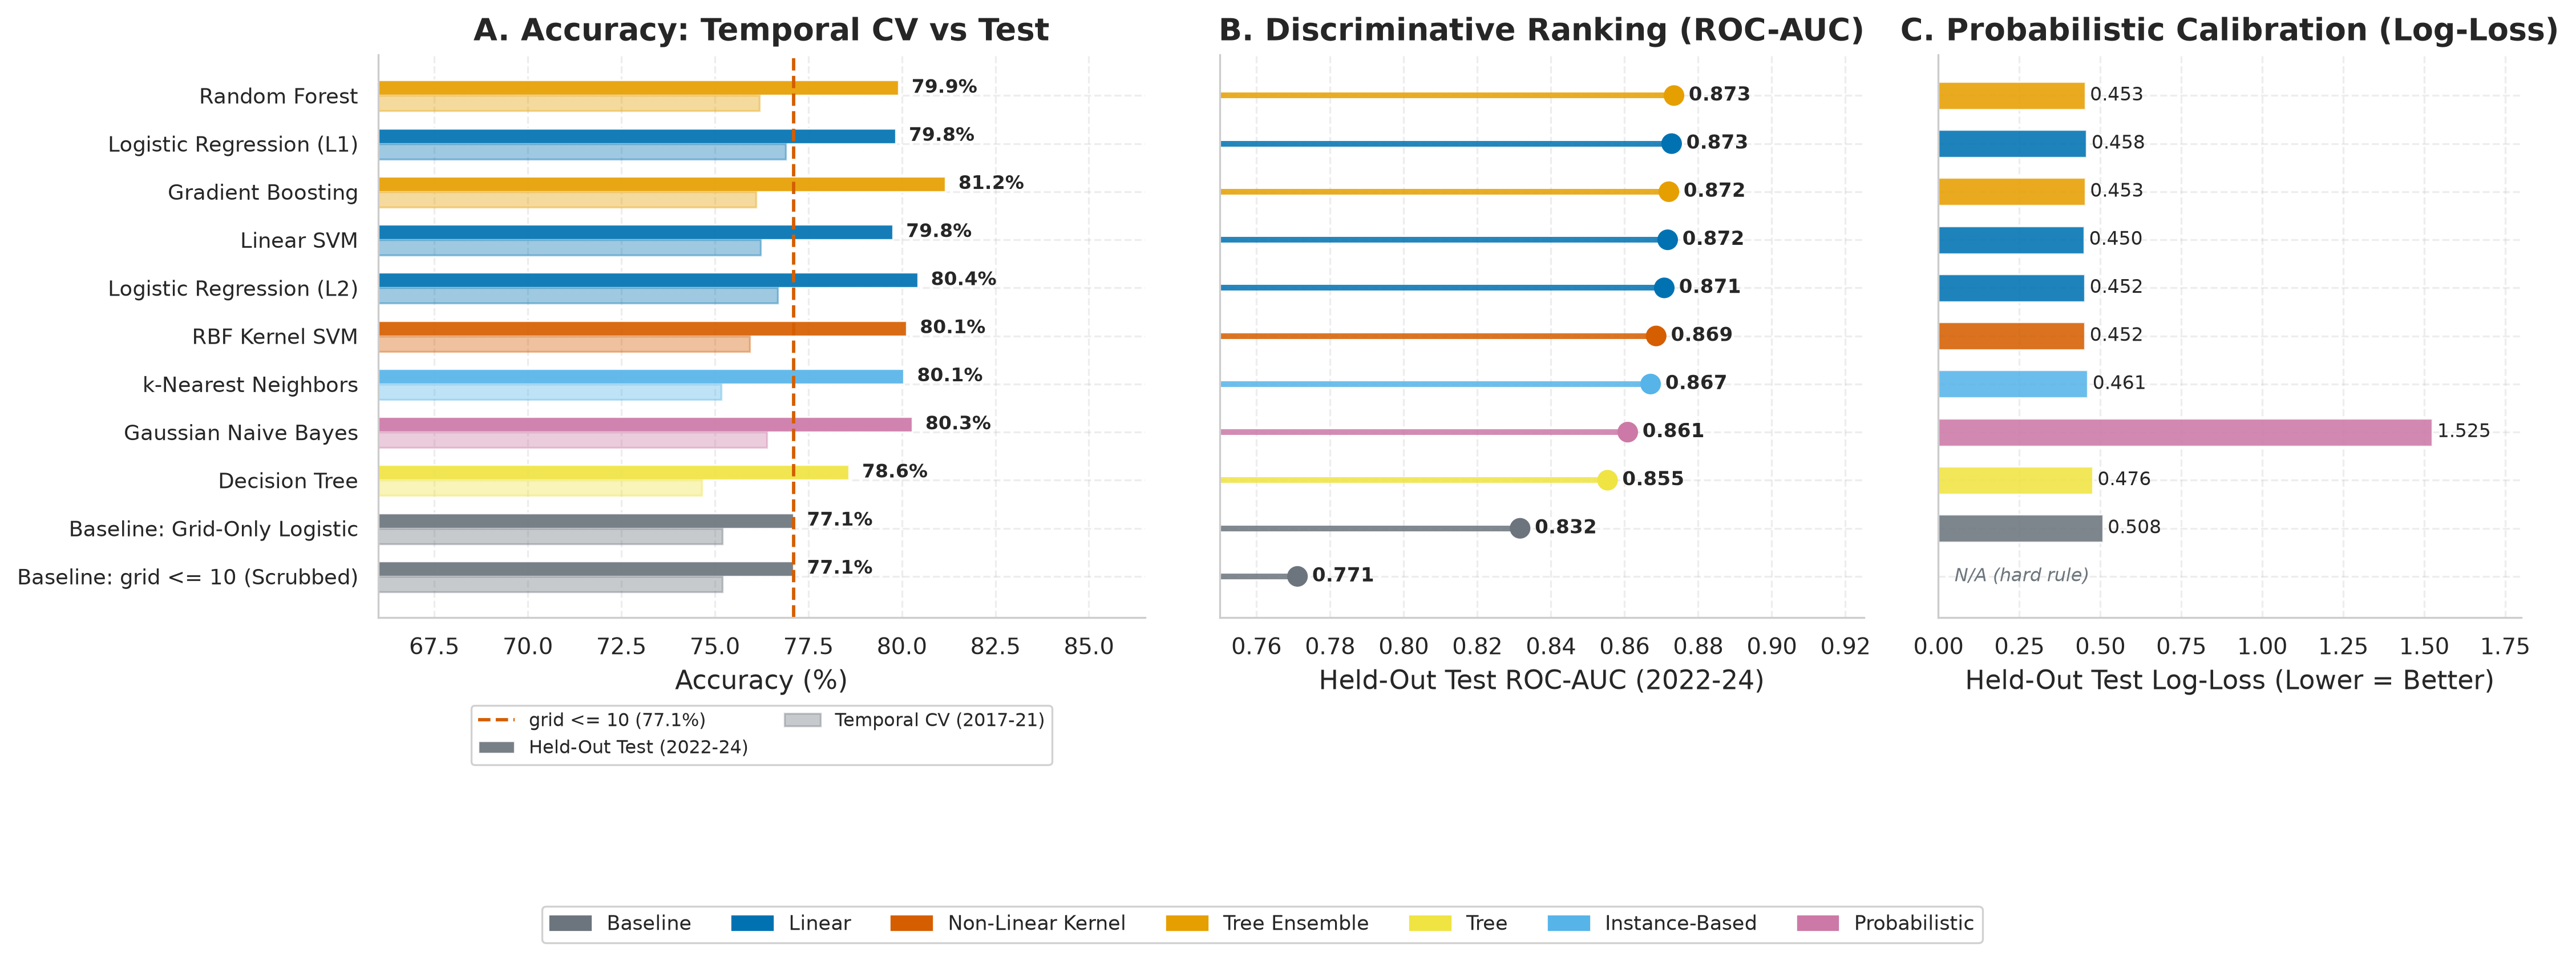
\includegraphics[width=0.94\textwidth]{figures/followup2/fig07_model_comparison_cv_vs_test.png}
  \caption{Model benchmark across Accuracy (A), ROC-AUC (B), and Log-Loss (C). Linear models match ensembles in AUC and lead calibration, whereas Gaussian NB suffers severe log-loss miscalibration (1.525) due to collinearity.}
  \label{fig:bench}
\end{figure*}

\begin{enumerate}
  \item \textbf{Race-Level Shifting (Zero Teammate Leakage):} Because two cars share a constructor and 20 cars share a circuit in race~$t$, naive row-wise \code{.shift(1)} leaks Car~\#1's race-$t$ finish into Car~\#2! We aggregate constructor and circuit streams to the \code{(entity, raceId)} race level and apply \code{.shift(1)} strictly before rolling/expanding computations. Points use the unified modern 25--18--\dots--1 scale (\code{modern\ub points\ub equiv}).
  \item \textbf{Empirical Bayes / MAP Smoothing (Lectures 5--6):} Sparse early rolling and circuit rates are shrunk toward fixed neutral priors via $(\sum y + m p_0)/(n + m)$ ($p_0=0.50$, $m\in\{2,3,4\}$) without peeking at dataset statistics. Non-negative \code{grid\ub penalty\ub drop} $= \max(0, \text{grid\ub clean} - \text{qualy\ub pos})$ avoids exact algebraic collinearity.
  \item \textbf{Automated Adversarial Leakage Audit:} \code{verify\ub no\ub leakage()} programmatically proves (i)~0 overlap with forbidden in-race columns, (ii)~bit-for-bit invariance (\code{max\ub abs\ub diff = 0.0}) of all 2010--2021 features when every 2022--2024 outcome is inverted, and (iii)~bit-for-bit invariance (\code{0.0}) of all 20 entries in probe race 2023 Round~10 when its own outcomes are inverted---while verifying Round~11 rolling features update (\code{diff = 5.83}).
\end{enumerate}

\subsection{Temporal Validation, Curriculum Models \& Statistical Testing}
All imputation (\code{SimpleImputer(\allowbreak{}median)}) and scaling (\code{Standard\allowbreak{}Scaler}) occur strictly inside \code{scikit-learn} \code{Pipeline}s. Hyperparameters are tuned exclusively via \textbf{5-fold Expanding-Window Seasonal CV} (validation seasons 2017--2021; fold~$k$ trains strictly on seasons $< y_k$) optimizing \textbf{ROC-AUC}, then evaluated once on held-out \textbf{2022--2024 Ground-Effect Test} ($n=1{,}359$). We benchmark \textbf{3 baselines} (Majority, Scrubbed \code{grid <= 10}, Grid-Only Logistic) against \textbf{9 course models}: L2 Ridge Logistic, L1 Lasso Logistic, Platt-calibrated Linear SVM, Gaussian Naive Bayes, k-NN, Platt-calibrated RBF SVM, Decision Tree (Entropy/Gini), Random Forest, and Gradient Boosting. Significance is evaluated via exact two-sided \textbf{McNemar tests} and \textbf{2,000-resample paired bootstrap 95\% CIs}.

% =========================================================================
% SECTION 4
% =========================================================================
\section{Experiments, 7-Subset Ablation \& ``What-If'' Studies}

\subsection{Full 12-Model Benchmark (Testing H2 \& H3)}
Table~\ref{tab:bench} and Figure~\ref{fig:bench} report temporal CV and held-out Test results across all 12 models.

% --- Floats declared on Page 3 -> Top of Page 4 ---
\begin{figure*}[t]
  \centering
  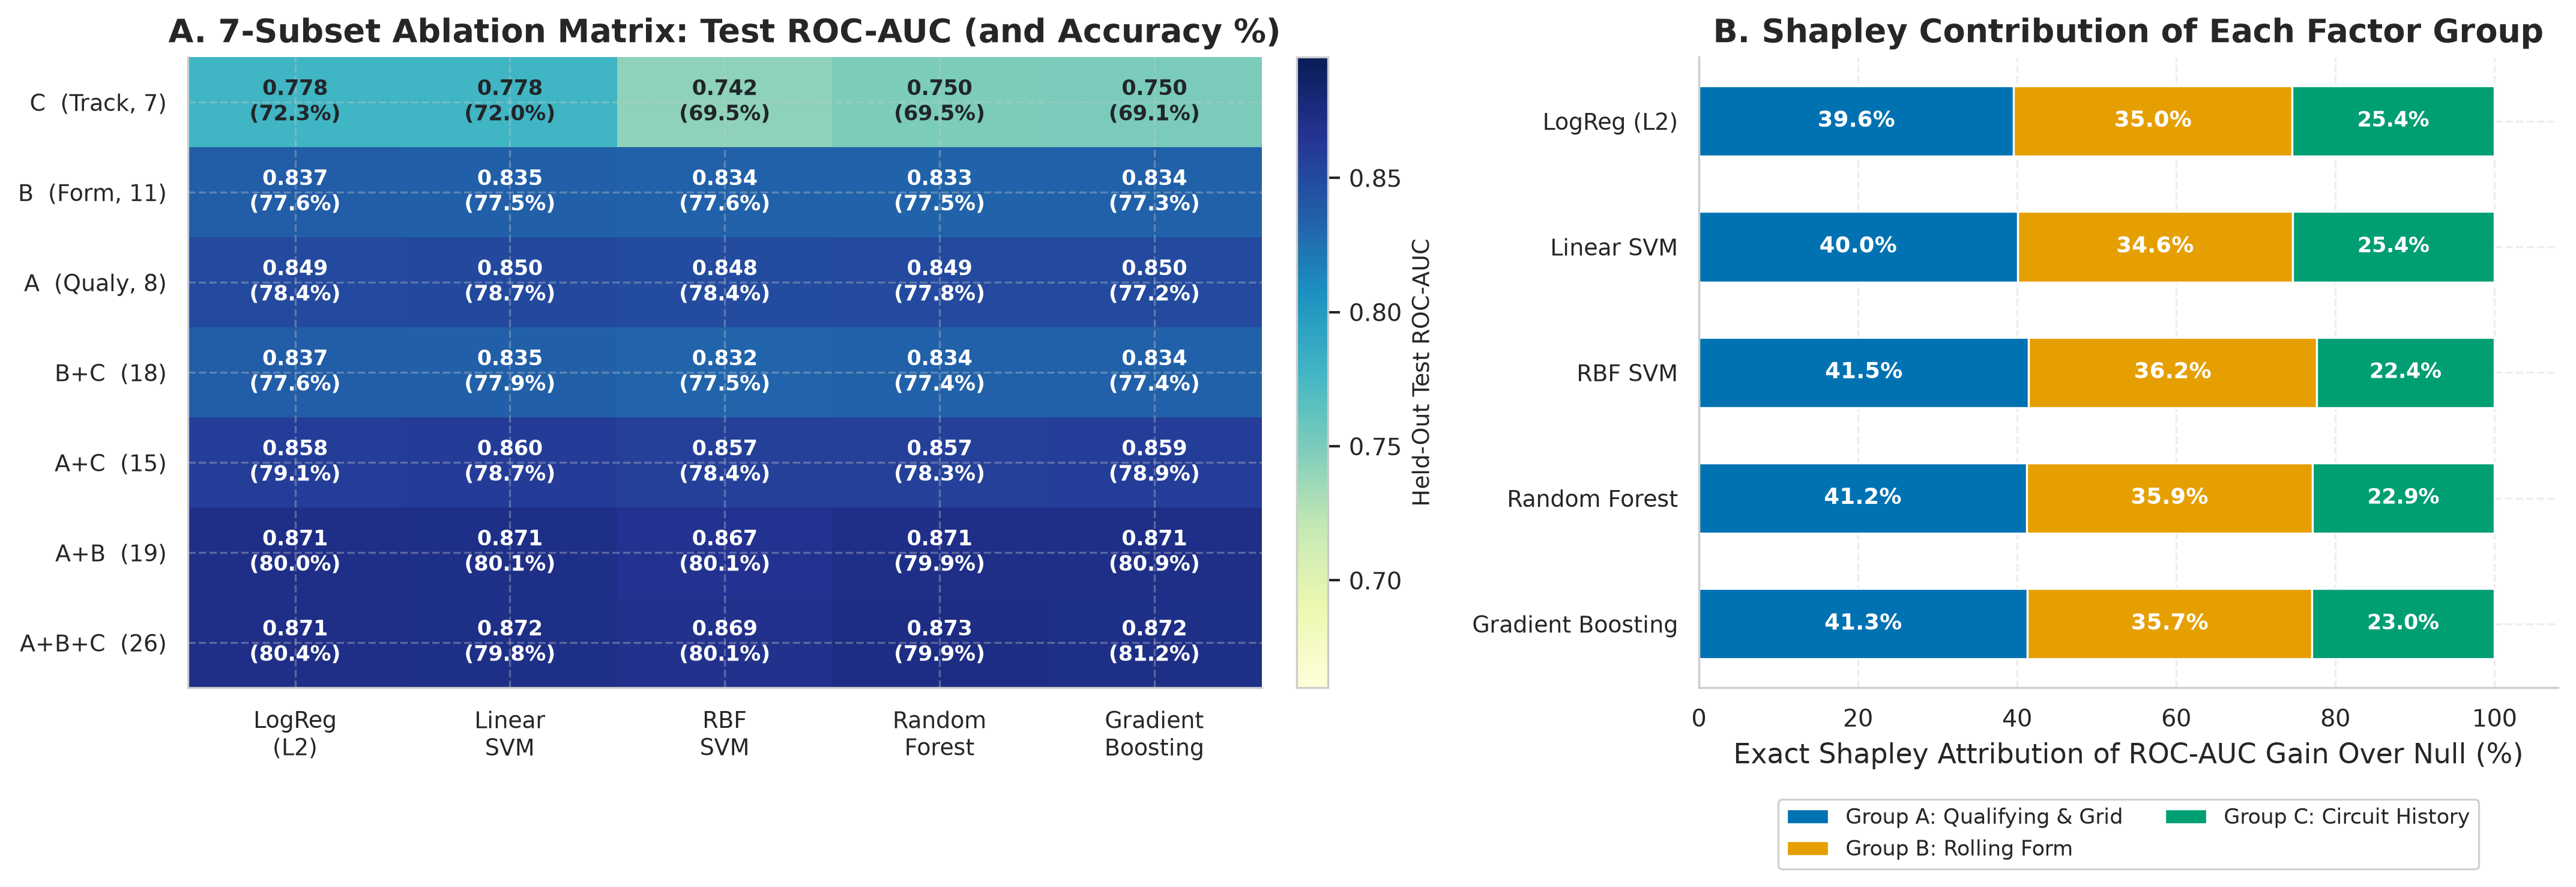
\includegraphics[width=0.90\textwidth]{figures/followup2/fig08_ablation_7subsets_and_shapley.png}
  \caption{Complete 7-subset ablation matrix (Test ROC-AUC and Accuracy \%) across 5 model families (A), and exact Shapley group attribution of ROC-AUC gain over null (B).}
  \label{fig:ablation}
\end{figure*}

\begin{figure*}[t]
  \centering
  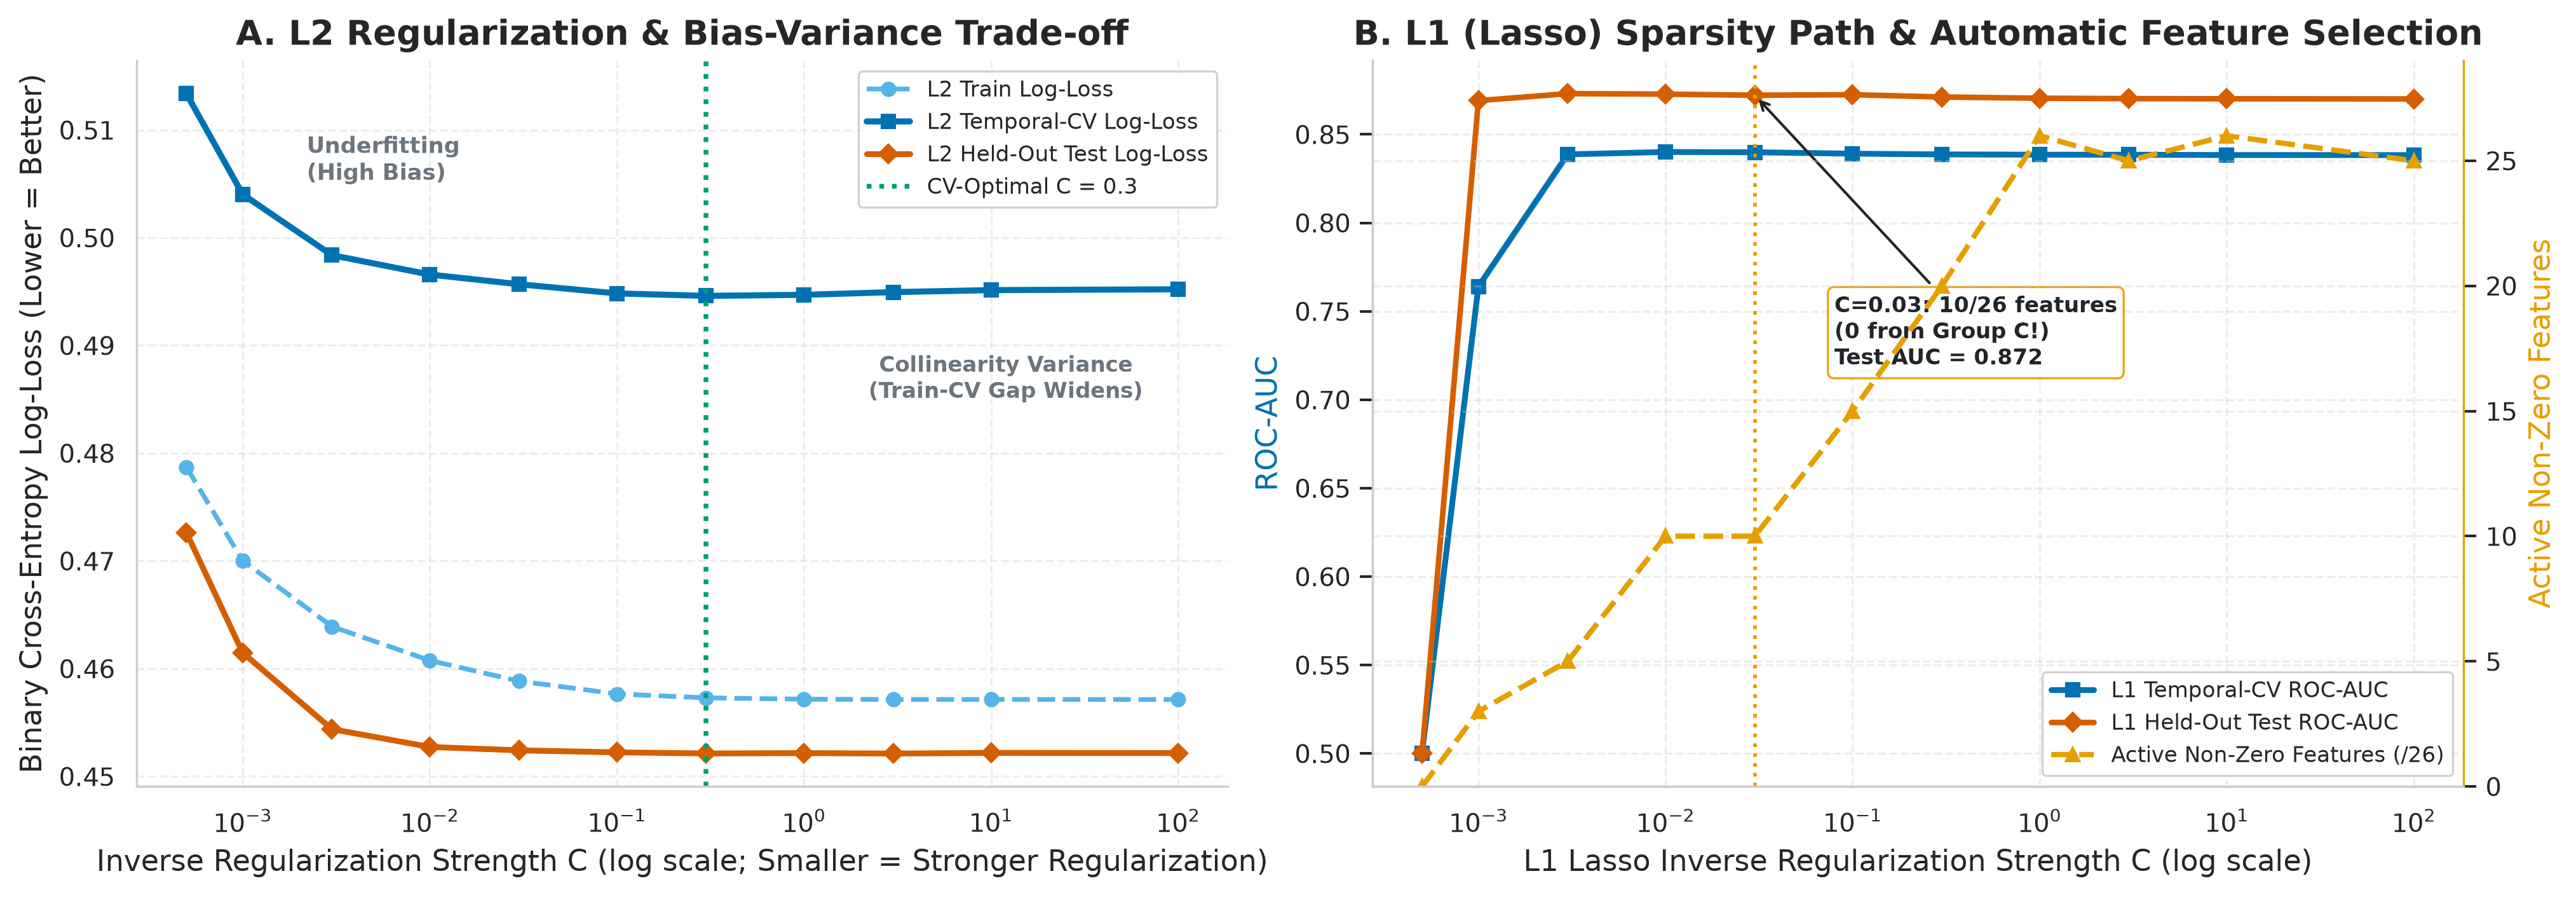
\includegraphics[width=0.90\textwidth]{figures/followup2/fig09_regularization_and_bias_variance.png}
  \caption{L2 bias-variance curve across inverse regularization~$C$ (A), and L1 Lasso sparsity path reaching near-peak Test AUC (0.872) with only 10/26 active features---zero from Group C (B).}
  \label{fig:reg}
\end{figure*}

\begin{figure*}[t]
  \centering
  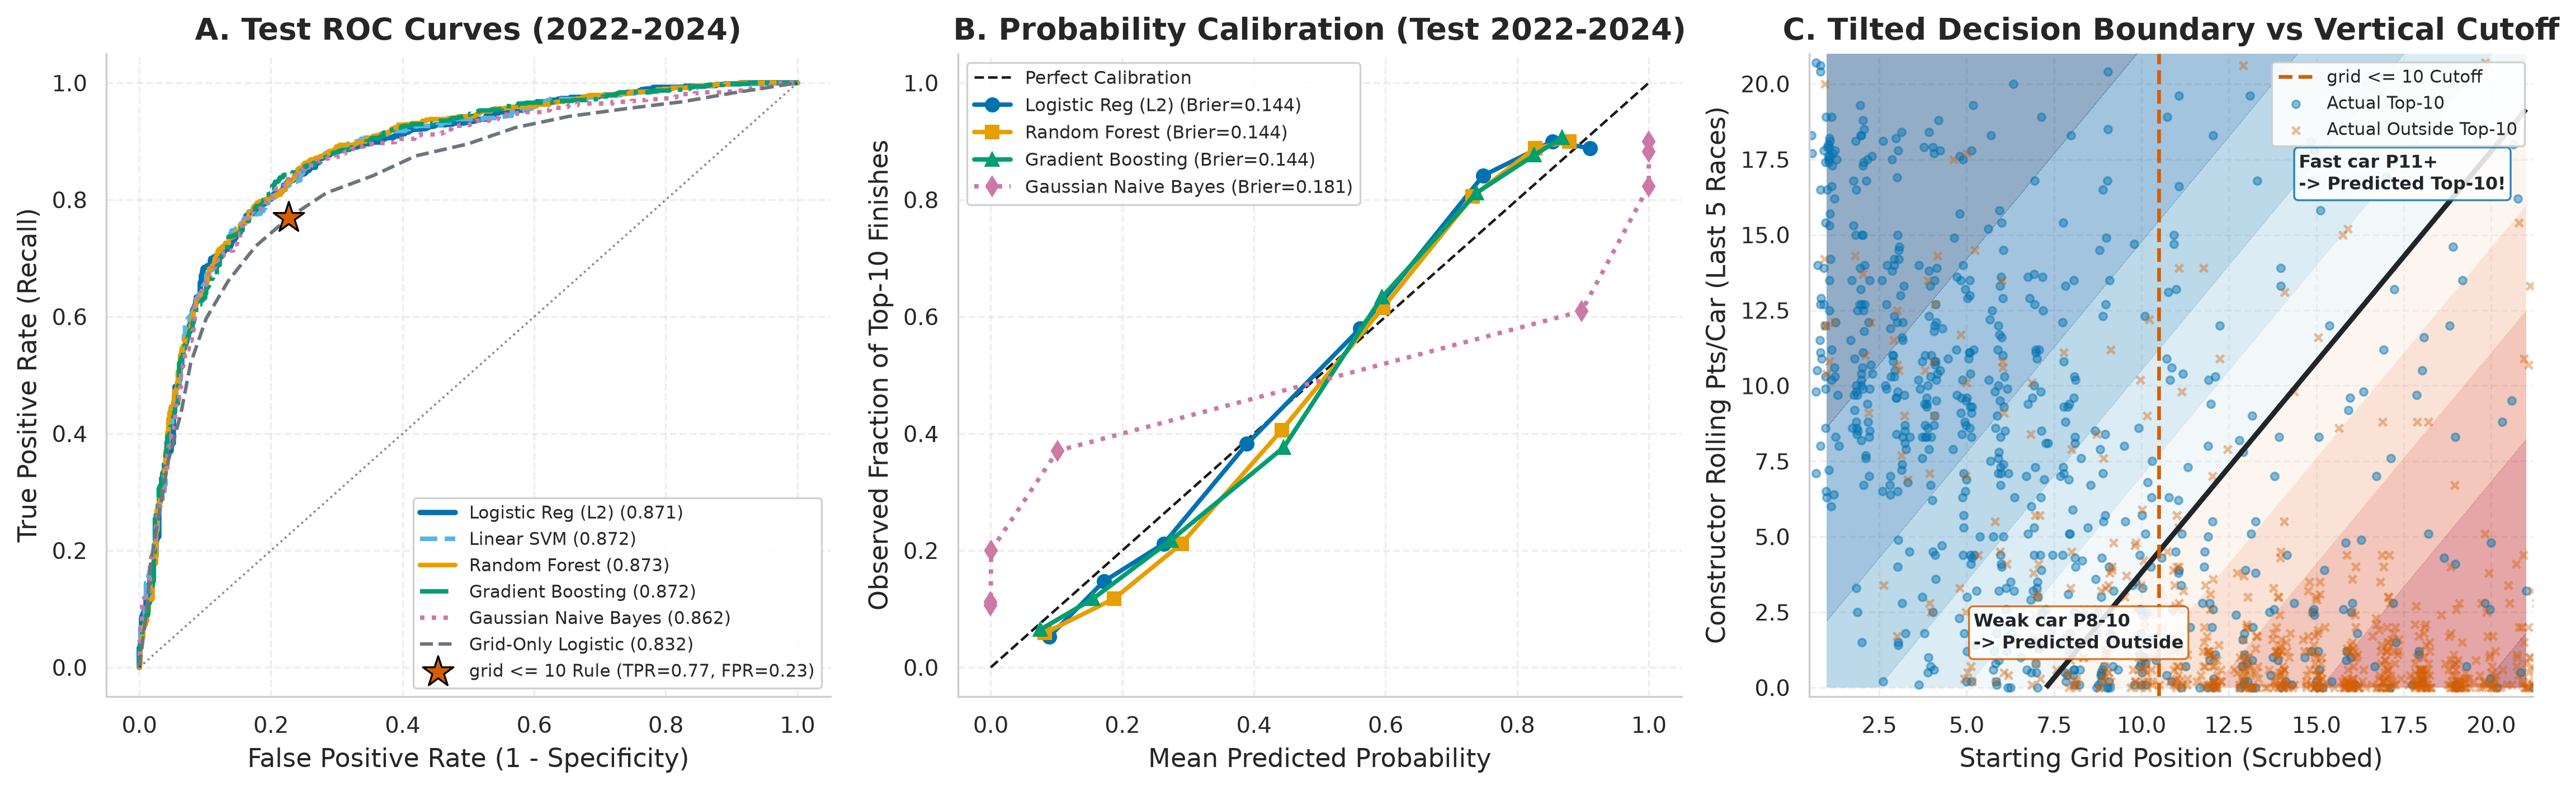
\includegraphics[width=0.92\textwidth]{figures/followup2/fig11_roc_pr_calibration_and_boundary.png}
  \caption{Test ROC curves vs.\ \code{grid <= 10} operating star (A), calibration curves contrasting linear/ensemble models with overconfident Gaussian NB (B), and tilted 2D linear boundary vs.\ vertical cutoff (C).}
  \label{fig:cal}
\end{figure*}

\begin{itemize}
  \item \textbf{Significant Baseline Lift (H3 Confirmed):} Every regularized linear, kernel, and ensemble model significantly beats \code{grid <= 10} (77.12\%, $p\le 0.009$). L2 Logistic adds \textbf{+3.31 pp} accuracy (95\% CI $[+1.47, +5.37]$ pp; 116 overturn wins vs.\ 71 losses) and \textbf{+0.0392} ROC-AUC over Grid-Only Logistic (95\% CI $[+0.0256, +0.0534]$, $p<0.001$).
  \item \textbf{Linear Parity with Ensembles (H2 Confirmed with Nuance):} \textbf{L1 Logistic} ranks \#1 in CV (\textbf{0.8401} AUC, \textbf{76.90\%} Acc) and statistically ties \textbf{Random Forest} on Test (McNemar $p=1.000$, 21 vs.\ 22 discordant pairs; $\Delta\text{AUC}=-0.0006$, 95\% CI $[-0.0043, +0.0030]$). \textbf{Linear SVM} achieves the best Test Log-Loss (\textbf{0.4504}) and Brier (\textbf{0.1428}) overall. \textbf{Gradient Boosting} edges ahead marginally in raw accuracy at $t=0.50$ (\textbf{81.16\%}) without improving AUC (0.8720) or calibration (0.4534).
  \item \textbf{Naive Bayes Calibration Breakdown (Lecture~5):} Gaussian NB achieves 80.28\% accuracy but catastrophic Log-Loss (\textbf{1.5255}, $>3\times$ Logistic) because feature collinearity breaks conditional independence, pushing posteriors to extreme 0/1 values (Figure~\ref{fig:cal}B).
\end{itemize}

\subsection{Centerpiece: 7-Subset Factor Group Ablation \& Exact Shapley Attribution (Testing H1)}
Retuning all $2^3 - 1 = 7$ non-empty subsets across 5 model families (35 temporal pipelines) and computing exact 3-player Shapley values ($\phi_A, \phi_B, \phi_C$; Figure~\ref{fig:ablation}) decisively confirms \textbf{H1}:
\begin{itemize}
  \item \textbf{Rolling Form (B) Drives a Universal Jump:} \code{A} $\rightarrow$ \code{A+B} boosts Test ROC-AUC by \textbf{+0.019 to +0.022} across every model family (LogReg L2: $0.8492 \rightarrow 0.8710$, Log-Loss $0.4872 \rightarrow 0.4514$; GradBoost Acc $+3.7$ pp).
  \item \textbf{Circuit History (C) Adds Negligible Marginal Value:} \code{A+B} $\rightarrow$ \code{A+B+C} changes Test AUC by \textbf{$-0.0002$} (LogReg L2), $+0.0005$ (Linear SVM), $+0.0010$ (GradBoost), and $+0.0025$ (RF). Standalone \code{C} reaches 0.75--0.78 AUC (22--25\% Shapley AUC share) solely as a \emph{lagged proxy for persistent team quality} when A and B are absent; once current form is included, circuit affinity is subsumed (Groups A+B capture \textbf{82.6\%--86.0\%} of Log-Loss Shapley reduction).
\end{itemize}

\subsection{``What-If'' Studies, Interpretability \& Decision Geometry}

% --- Floats declared on Page 4 -> Top of Page 5 ---
\begin{figure*}[t]
  \centering
  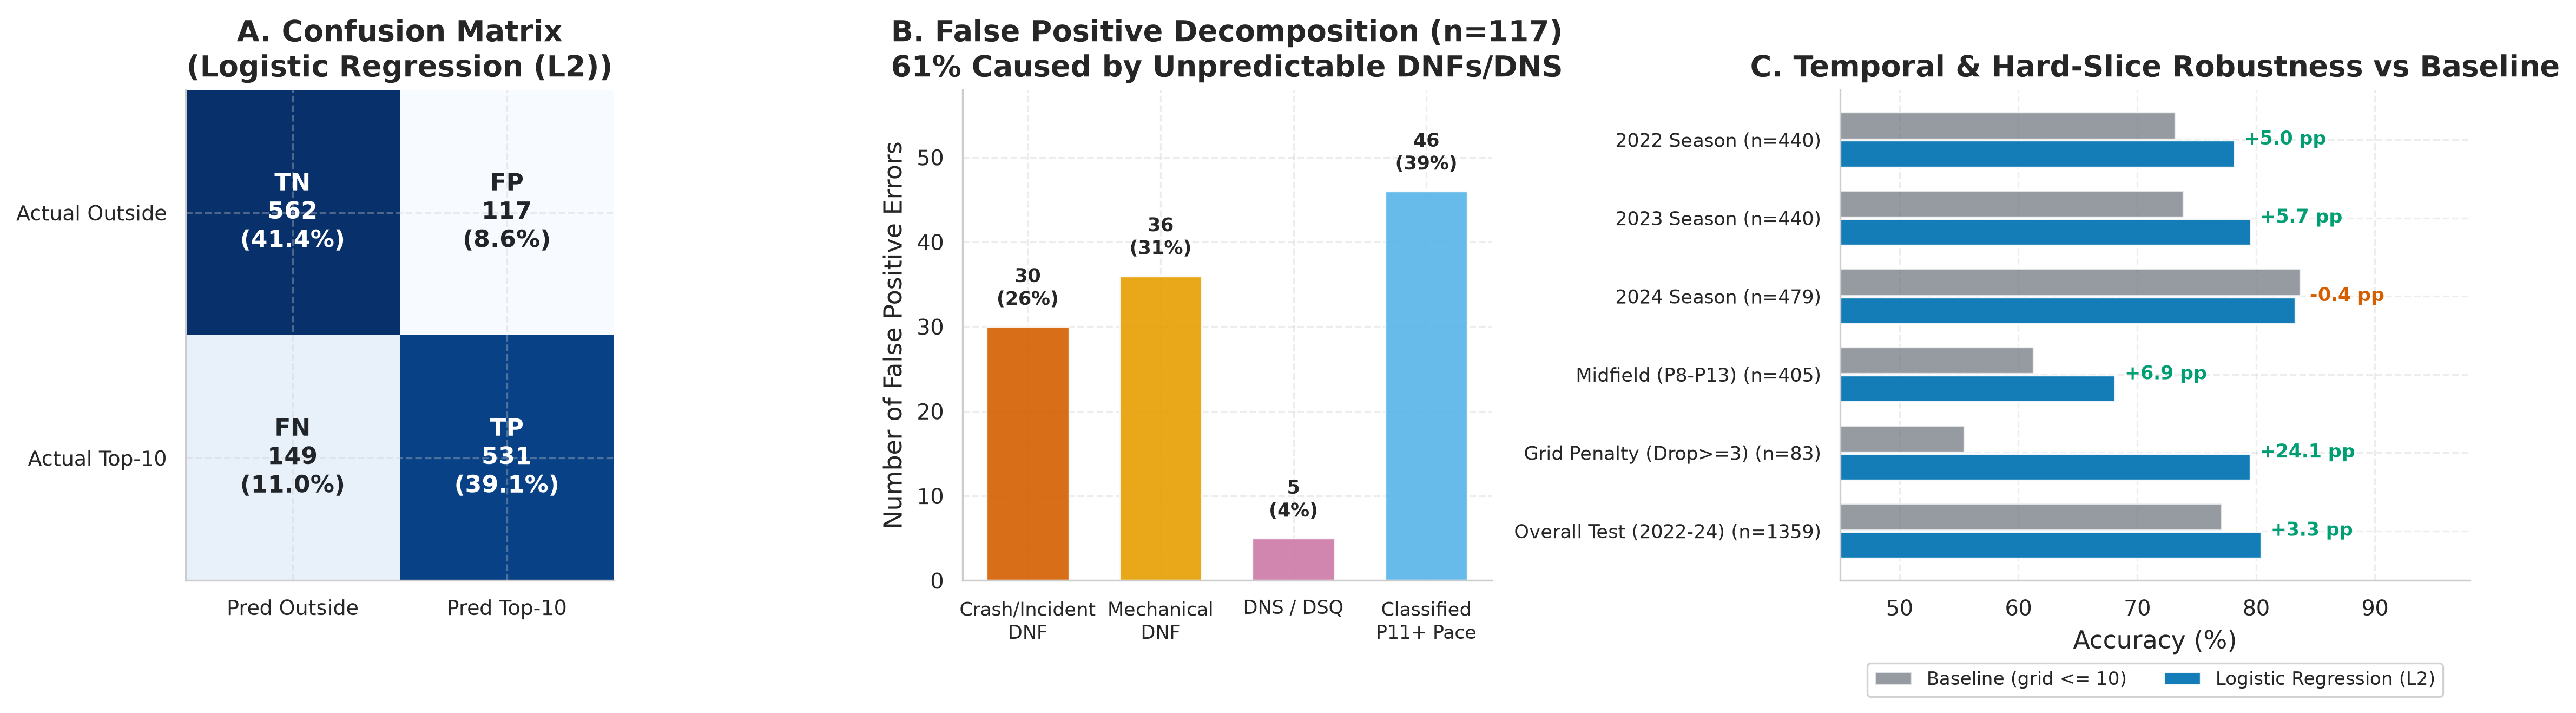
\includegraphics[width=0.95\textwidth]{figures/followup2/fig12_error_analysis_and_regime_robustness.png}
  \caption{Confusion matrix (A), post-hoc False Positive decomposition exposing 60.7\% irreducible DNF/DNS errors (B), and slice gains showing +24.1 pp on Grid Penalty Drops and +6.9 pp in the Midfield Zone (C).}
  \label{fig:err}
\end{figure*}

\begin{table*}[t]
  \centering
  \caption{Representative 2022--2024 test case studies: confident overturn wins against \code{grid <= 10} (top) vs.\ highest-confidence irreducible DNF/chaos misses (bottom).}
  \label{tab:cases}
  {\scriptsize
  \setlength{\tabcolsep}{4.6pt}
  \renewcommand{\arraystretch}{1.14}
  \begin{tabularx}{\textwidth}{l l l c c c c L}
    \toprule
    \textbf{Type} & \textbf{Grand Prix} & \textbf{Driver (Team)} & \textbf{Grid / Q} & \textbf{Fin.} & \textbf{L2 $P$} & \textbf{Rule} & \textbf{Domain Mechanism} \\
    \midrule
    Win & 2024 Belgian GP & M. Verstappen (Red Bull) & P11 / Q1 & P4 & \textbf{86.9\%} & Fail & Engine penalty; dominant race pace \\
    Win & 2022 Belgian GP & M. Verstappen (Red Bull) & P14 / Q1 & P1 & \textbf{82.1\%} & Fail & Engine penalty; wins from P14 \\
    Win & 2022 Italian GP & N. Latifi (Williams) & P10 / Q16 & P15 & \textbf{13.5\%} & Fail & Promoted by others' penalties \\
    Win & 2023 Dutch GP & L. Sargeant (Williams) & P10 / Q10 & P20 & \textbf{15.8\%} & Fail & Weak team form (1.0 pts/car) \\
    \midrule
    Miss & 2024 Australian GP & M. Verstappen (Red Bull) & P1 / Q1 & DNF & 93.1\% & Fail & Mechanical DNF (Brakes fire) \\
    Miss & 2022 Azerbaijan GP & C. Leclerc (Ferrari) & P1 / Q1 & DNF & 92.8\% & Fail & Mechanical DNF (Power Unit) \\
    Miss & 2022 US GP (COTA) & C. Sainz (Ferrari) & P1 / Q1 & DNF & 91.8\% & Fail & Lap-1 Turn-1 collision damage \\
    Miss & 2023 Qatar GP & G. Zhou (Alfa Romeo) & P19 / Q19 & P9 & 7.7\% & Pass & Multi-DNF / tyre strategy surge \\
    \bottomrule
  \end{tabularx}}
\end{table*}

\begin{enumerate}
  \item \textbf{Regularization \& L1 Automatic Group Elimination (Figure~\ref{fig:reg}):} Sweeping $C \in [5\times 10^{-4}, 10^2]$ exposes high-bias underfitting at small $C$ and widening train--CV variance at large $C$. At CV-optimal \textbf{L1 $C=0.01$} (Test AUC \textbf{0.8728}), Lasso keeps only \textbf{10/26 features}: \textbf{4 from Group~A}, \textbf{6 from Group~B}, and \textbf{0/7 from Group~C}---an independent confirmation of H1!
  \item \textbf{Rolling Horizon ($W \in \{3, 5, 10\}$) \& Lineages:} Longer windows ($W=10$: Test AUC \textbf{0.8751}, Acc \textbf{80.35\%}, Log-Loss 0.4550) beat reactive $W=3$ (AUC 0.8702, Log-Loss 0.4628) by dampening per-race DNF noise. Canonical lineages improve CV AUC ($0.8397 \rightarrow 0.8401$) and rebranded-team 2022--24 Test calibration (Log-Loss $0.5152 \rightarrow 0.5132$, AUC $0.8054 \rightarrow 0.8078$).
  \item \textbf{CV Threshold Calibration:} Tuning the cutoff strictly on 2017--2021 OOF CV ($t=0.455$, reflecting the 46.7\% Dev vs.\ 50.0\% 20-car Test base rate) raises L1 Logistic Test Accuracy from \textbf{79.84\% $\rightarrow$ 80.35\%} and F1 from \textbf{0.796 $\rightarrow$ 0.810}.
  \item \textbf{Interpretability \& 2D Geometry (Figure~\ref{fig:cal}):} Out-of-sample permutation importance confirms both L2 Logistic and Random Forest rely primarily on \code{const\ub roll10\ub avg\ub pos}, \code{drv\ub roll5\ub avg\ub pos}, \code{qualy\ub pos}, and \code{grid\ub pct}, with near-zero drop for Group~C. In L2 Logistic, collinearity induces a classic suppressor sign-flip on \code{const\ub roll5\ub pts\ub per\ub car} ($-0.62$, podium-skewness contrast against avg position), which L1 sparsity cleanly removes. Figure~\ref{fig:cal}C illustrates how the tilted linear boundary overturns the vertical \code{grid <= 10} rule in both opposite corners.
\end{enumerate}

% =========================================================================
% SECTION 5
% =========================================================================
\section{Critical Appraisal, Error Analysis \& Conclusion}

\subsection{Hard-Slice Gains, Bayes Error Floor \& 2024 Appraisal}
Figure~\ref{fig:err} and Table~\ref{tab:cases} dissect our L2 Logistic model's hard-slice gains and irreducible failure modes across 2022--2024:
\begin{itemize}
  \item \textbf{Hard-Slice Triumphs:} On \textbf{Grid Penalty Drops ($\ge 3$ places, $n=83$)}, \code{grid <= 10} falls to \textbf{55.4\%}, while L2 Logistic reaches \textbf{79.5\%} (\textbf{+24.1 pp}, AUC 0.873), overturning Verstappen's P11/P14 Spa recoveries and Leclerc's P12 COTA podium while demoting penalty-promoted backmarkers (Latifi P10 $\rightarrow$ P15, Monza 2022). In the \textbf{P8--P13 Midfield ($n=405$)}, accuracy jumps \textbf{+6.9 pp} ($61.2\% \rightarrow 68.1\%$).
  \item \textbf{Quantifying the Irreducible Bayes Error Ceiling:} Post-hoc inspection of all 117 False Positives proves that \textbf{60.7\% (71/117)} stem from unpredictable race-day retirements---30 Crash/Incident DNFs (26\%), 36 Mechanical DNFs (31\%), and 5 DNS/DSQ (4\%)---leaving only \textbf{46 classified P11+ pace misses} (3.4\% of all starts!). Similarly, \textbf{46.3\% (69/149)} of False Negatives occur in high-attrition races ($\ge 2$ Top-10 DNFs). Table~\ref{tab:cases} illustrates pole-sitters retiring with brake, turbo, power-unit, or Lap-1 collision failures despite $P(\text{Top-10}) > 91\%$.
  \item \textbf{Honest 2024 Regime Appraisal:} L2 Logistic beats \code{grid <= 10} by \textbf{+5.0 pp} in 2022 and \textbf{+5.7 pp} in 2023, yet trails marginally by $-0.4$ pp in 2024 (83.7\% vs.\ 83.3\%, despite \textbf{0.910} ROC-AUC), reflecting 2024's 15-year-low mechanical DNF rate (11.3\%) and tight four-team pace convergence.
\end{itemize}

\subsection{Conclusion \& Future Work}
Rigorous scrubbing, zero-leakage temporal validation, and 7-subset ablation yield three core conclusions: (1)~\textbf{Qualifying context and rolling momentum explain nearly 100\% of predictable pre-race Top-10 variance}, while historical circuit affinity adds negligible marginal lift and is dropped 7/7 by L1 Lasso; (2)~\textbf{Regularized linear models (L1/L2 Logistic, Linear SVM) tie Random Forest in ranking and lead in calibration}, delivering $+3.3$ pp overall and $+24.1$ pp grid-penalty gains over \code{grid <= 10} with full interpretability; and (3)~\textbf{60.7\% of False Positives arise from irreducible race-day retirements}, establishing a natural pre-race accuracy ceiling near 81--84\%. Future work should integrate strictly pre-race FastF1 Friday FP2 long-run pace, FIA tyre nominations, and weather forecasts to narrow the remaining 39\% classified-finish gap without introducing in-race leakage.

\section*{References}
\begin{enumerate}[label={[\arabic*]}, leftmargin=1.5em, itemsep=1.5pt, topsep=2pt, font=\footnotesize]
  \item {\footnotesize Rohan Rao / Ergast API, \textit{Formula 1 World Championship (1950--2024)}, Kaggle.}
  \item {\footnotesize Pedregosa et al.\ (2011), \textit{Scikit-learn}, JMLR 12:2825--2830.}
  \item {\footnotesize Shapley, L.S.\ (1953), \textit{A Value for $n$-Person Games}.}
  \item {\footnotesize Karatzas, D. \& Mulayim, O.\ (2026), \textit{Fundamentals of Machine Learning (L1--L11)}, UAB.}
\end{enumerate}

\end{document}
